\documentclass[]{ximera}
%handout:  for handout version with no solutions or instructor notes
%handout,instructornotes:  for instructor version with just problems and notes, no solutions
%noinstructornotes:  shows only problem and solutions

%% handout
%% space
%% newpage
%% numbers
%% nooutcomes

%I added the commands here so that I would't have to keep looking them up
%\newcommand{\RR}{\mathbb R}
%\renewcommand{\d}{\,d}
%\newcommand{\dd}[2][]{\frac{d #1}{d #2}}
%\renewcommand{\l}{\ell}
%\newcommand{\ddx}{\frac{d}{dx}}
%\everymath{\displaystyle}
%\newcommand{\dfn}{\textbf}
%\newcommand{\eval}[1]{\bigg[ #1 \bigg]}

%\begin{image}
%\includegraphics[trim= 170 420 250 180]{Figure1.pdf}
%\end{image}

%add a ``.'' below when used in a specific directory.

%\usepackage{todonotes}
%\usepackage{mathtools} %% Required for wide table Curl and Greens
%\usepackage{cuted} %% Required for wide table Curl and Greens
\newcommand{\todo}{}

\usepackage{esint} % for \oiint
\ifxake%%https://math.meta.stackexchange.com/questions/9973/how-do-you-render-a-closed-surface-double-integral
\renewcommand{\oiint}{{\large\bigcirc}\kern-1.56em\iint}
\fi


\graphicspath{
  {./}
  {ximeraTutorial/}
  {basicPhilosophy/}
  {functionsOfSeveralVariables/}
  {normalVectors/}
  {lagrangeMultipliers/}
  {vectorFields/}
  {greensTheorem/}
  {shapeOfThingsToCome/}
  {dotProducts/}
  {partialDerivativesAndTheGradientVector/}
  {../productAndQuotientRules/exercises/}
  {../normalVectors/exercisesParametricPlots/}
  {../continuityOfFunctionsOfSeveralVariables/exercises/}
  {../partialDerivativesAndTheGradientVector/exercises/}
  {../directionalDerivativeAndChainRule/exercises/}
  {../commonCoordinates/exercisesCylindricalCoordinates/}
  {../commonCoordinates/exercisesSphericalCoordinates/}
  {../greensTheorem/exercisesCurlAndLineIntegrals/}
  {../greensTheorem/exercisesDivergenceAndLineIntegrals/}
  {../shapeOfThingsToCome/exercisesDivergenceTheorem/}
  {../greensTheorem/}
  {../shapeOfThingsToCome/}
  {../separableDifferentialEquations/exercises/}
  {vectorFields/}
}

\newcommand{\mooculus}{\textsf{\textbf{MOOC}\textnormal{\textsf{ULUS}}}}

\usepackage{tkz-euclide}\usepackage{tikz}
\usepackage{tikz-cd}
\usetikzlibrary{arrows}
\tikzset{>=stealth,commutative diagrams/.cd,
  arrow style=tikz,diagrams={>=stealth}} %% cool arrow head
\tikzset{shorten <>/.style={ shorten >=#1, shorten <=#1 } } %% allows shorter vectors

\usetikzlibrary{backgrounds} %% for boxes around graphs
\usetikzlibrary{shapes,positioning}  %% Clouds and stars
\usetikzlibrary{matrix} %% for matrix
\usepgfplotslibrary{polar} %% for polar plots
\usepgfplotslibrary{fillbetween} %% to shade area between curves in TikZ
\usetkzobj{all}
\usepackage[makeroom]{cancel} %% for strike outs
%\usepackage{mathtools} %% for pretty underbrace % Breaks Ximera
%\usepackage{multicol}
\usepackage{pgffor} %% required for integral for loops



%% http://tex.stackexchange.com/questions/66490/drawing-a-tikz-arc-specifying-the-center
%% Draws beach ball
\tikzset{pics/carc/.style args={#1:#2:#3}{code={\draw[pic actions] (#1:#3) arc(#1:#2:#3);}}}



\usepackage{array}
\setlength{\extrarowheight}{+.1cm}
\newdimen\digitwidth
\settowidth\digitwidth{9}
\def\divrule#1#2{
\noalign{\moveright#1\digitwidth
\vbox{\hrule width#2\digitwidth}}}





\newcommand{\RR}{\mathbb R}
\newcommand{\R}{\mathbb R}
\newcommand{\N}{\mathbb N}
\newcommand{\Z}{\mathbb Z}

\newcommand{\sagemath}{\textsf{SageMath}}


%\renewcommand{\d}{\,d\!}
\renewcommand{\d}{\mathop{}\!d}
\newcommand{\dd}[2][]{\frac{\d #1}{\d #2}}
\newcommand{\pp}[2][]{\frac{\partial #1}{\partial #2}}
\renewcommand{\l}{\ell}
\newcommand{\ddx}{\frac{d}{\d x}}

\newcommand{\zeroOverZero}{\ensuremath{\boldsymbol{\tfrac{0}{0}}}}
\newcommand{\inftyOverInfty}{\ensuremath{\boldsymbol{\tfrac{\infty}{\infty}}}}
\newcommand{\zeroOverInfty}{\ensuremath{\boldsymbol{\tfrac{0}{\infty}}}}
\newcommand{\zeroTimesInfty}{\ensuremath{\small\boldsymbol{0\cdot \infty}}}
\newcommand{\inftyMinusInfty}{\ensuremath{\small\boldsymbol{\infty - \infty}}}
\newcommand{\oneToInfty}{\ensuremath{\boldsymbol{1^\infty}}}
\newcommand{\zeroToZero}{\ensuremath{\boldsymbol{0^0}}}
\newcommand{\inftyToZero}{\ensuremath{\boldsymbol{\infty^0}}}



\newcommand{\numOverZero}{\ensuremath{\boldsymbol{\tfrac{\#}{0}}}}
\newcommand{\dfn}{\textbf}
%\newcommand{\unit}{\,\mathrm}
\newcommand{\unit}{\mathop{}\!\mathrm}
\newcommand{\eval}[1]{\bigg[ #1 \bigg]}
\newcommand{\seq}[1]{\left( #1 \right)}
\renewcommand{\epsilon}{\varepsilon}
\renewcommand{\phi}{\varphi}


\renewcommand{\iff}{\Leftrightarrow}

\DeclareMathOperator{\arccot}{arccot}
\DeclareMathOperator{\arcsec}{arcsec}
\DeclareMathOperator{\arccsc}{arccsc}
\DeclareMathOperator{\si}{Si}
\DeclareMathOperator{\scal}{scal}
\DeclareMathOperator{\sign}{sign}


%% \newcommand{\tightoverset}[2]{% for arrow vec
%%   \mathop{#2}\limits^{\vbox to -.5ex{\kern-0.75ex\hbox{$#1$}\vss}}}
\newcommand{\arrowvec}[1]{{\overset{\rightharpoonup}{#1}}}
%\renewcommand{\vec}[1]{\arrowvec{\mathbf{#1}}}
\renewcommand{\vec}[1]{{\overset{\boldsymbol{\rightharpoonup}}{\mathbf{#1}}}\hspace{0in}}

\newcommand{\point}[1]{\left(#1\right)} %this allows \vector{ to be changed to \vector{ with a quick find and replace
\newcommand{\pt}[1]{\mathbf{#1}} %this allows \vec{ to be changed to \vec{ with a quick find and replace
\newcommand{\Lim}[2]{\lim_{\point{#1} \to \point{#2}}} %Bart, I changed this to point since I want to use it.  It runs through both of the exercise and exerciseE files in limits section, which is why it was in each document to start with.

\DeclareMathOperator{\proj}{\mathbf{proj}}
\newcommand{\veci}{{\boldsymbol{\hat{\imath}}}}
\newcommand{\vecj}{{\boldsymbol{\hat{\jmath}}}}
\newcommand{\veck}{{\boldsymbol{\hat{k}}}}
\newcommand{\vecl}{\vec{\boldsymbol{\l}}}
\newcommand{\uvec}[1]{\mathbf{\hat{#1}}}
\newcommand{\utan}{\mathbf{\hat{t}}}
\newcommand{\unormal}{\mathbf{\hat{n}}}
\newcommand{\ubinormal}{\mathbf{\hat{b}}}

\newcommand{\dotp}{\bullet}
\newcommand{\cross}{\boldsymbol\times}
\newcommand{\grad}{\boldsymbol\nabla}
\newcommand{\divergence}{\grad\dotp}
\newcommand{\curl}{\grad\cross}
%\DeclareMathOperator{\divergence}{divergence}
%\DeclareMathOperator{\curl}[1]{\grad\cross #1}
\newcommand{\lto}{\mathop{\longrightarrow\,}\limits}

\renewcommand{\bar}{\overline}

\colorlet{textColor}{black}
\colorlet{background}{white}
\colorlet{penColor}{blue!50!black} % Color of a curve in a plot
\colorlet{penColor2}{red!50!black}% Color of a curve in a plot
\colorlet{penColor3}{red!50!blue} % Color of a curve in a plot
\colorlet{penColor4}{green!50!black} % Color of a curve in a plot
\colorlet{penColor5}{orange!80!black} % Color of a curve in a plot
\colorlet{penColor6}{yellow!70!black} % Color of a curve in a plot
\colorlet{fill1}{penColor!20} % Color of fill in a plot
\colorlet{fill2}{penColor2!20} % Color of fill in a plot
\colorlet{fillp}{fill1} % Color of positive area
\colorlet{filln}{penColor2!20} % Color of negative area
\colorlet{fill3}{penColor3!20} % Fill
\colorlet{fill4}{penColor4!20} % Fill
\colorlet{fill5}{penColor5!20} % Fill
\colorlet{gridColor}{gray!50} % Color of grid in a plot

\newcommand{\surfaceColor}{violet}
\newcommand{\surfaceColorTwo}{redyellow}
\newcommand{\sliceColor}{greenyellow}




\pgfmathdeclarefunction{gauss}{2}{% gives gaussian
  \pgfmathparse{1/(#2*sqrt(2*pi))*exp(-((x-#1)^2)/(2*#2^2))}%
}


%%%%%%%%%%%%%
%% Vectors
%%%%%%%%%%%%%

%% Simple horiz vectors
\renewcommand{\vector}[1]{\left\langle #1\right\rangle}


%% %% Complex Horiz Vectors with angle brackets
%% \makeatletter
%% \renewcommand{\vector}[2][ , ]{\left\langle%
%%   \def\nextitem{\def\nextitem{#1}}%
%%   \@for \el:=#2\do{\nextitem\el}\right\rangle%
%% }
%% \makeatother

%% %% Vertical Vectors
%% \def\vector#1{\begin{bmatrix}\vecListA#1,,\end{bmatrix}}
%% \def\vecListA#1,{\if,#1,\else #1\cr \expandafter \vecListA \fi}

%%%%%%%%%%%%%
%% End of vectors
%%%%%%%%%%%%%

%\newcommand{\fullwidth}{}
%\newcommand{\normalwidth}{}



%% makes a snazzy t-chart for evaluating functions
%\newenvironment{tchart}{\rowcolors{2}{}{background!90!textColor}\array}{\endarray}

%%This is to help with formatting on future title pages.
\newenvironment{sectionOutcomes}{}{}



%% Flowchart stuff
%\tikzstyle{startstop} = [rectangle, rounded corners, minimum width=3cm, minimum height=1cm,text centered, draw=black]
%\tikzstyle{question} = [rectangle, minimum width=3cm, minimum height=1cm, text centered, draw=black]
%\tikzstyle{decision} = [trapezium, trapezium left angle=70, trapezium right angle=110, minimum width=3cm, minimum height=1cm, text centered, draw=black]
%\tikzstyle{question} = [rectangle, rounded corners, minimum width=3cm, minimum height=1cm,text centered, draw=black]
%\tikzstyle{process} = [rectangle, minimum width=3cm, minimum height=1cm, text centered, draw=black]
%\tikzstyle{decision} = [trapezium, trapezium left angle=70, trapezium right angle=110, minimum width=3cm, minimum height=1cm, text centered, draw=black]


\author{Jim Talamo}

\outcome{Determine whether a given ODE is separable.}
\outcome{Solve separable equations.}
\outcome{Make a conjecture about solutions to an IVP from a direction field then verify them by solving the equation.}

\title{Separable Equations}

\begin{document}
\begin{abstract}
\end{abstract}
\maketitle

\vspace{-0.9in}

\section{Discussion Questions}

\begin{problem} 

Determine which of the following ODE are separable.

\begin{tabular}{llll}

I. $y'=e^{2x+3y}$ \qquad & II. $x \dfrac{dy}{dx} =\ln(2xy^2)$ \qquad & III. $y^2 \dfrac{dy}{dx} = x^2-x^2\sin(y)$ \qquad & IV. $\dfrac{dy}{dx} +4xy =x^2$ 
\end{tabular}

\begin{solution}
An ODE is separable if it can be rewritten as $\frac{dy}{dx} = f(x) \cdot g(y)$. 

I. This equation is separable, since it can be written as 
$$
\frac{dy}{dx} = e^{2x} \cdot e^{3y}.
$$

II. This equation is not separable.

III. Rewriting the equation, we have 
$$
\frac{dy}{dx} = x^2 \cdot \frac{1-\sin(y)}{y^2}.
$$
The equation is therefore separable.

IV. This equation is not separable.
\end{solution}
\end{problem}


%%%%%%%%%%%%%%%%%%%%

\begin{problem} 

A student claims that the  general solution to the differential equation $y' = 2x+8y^3$ is $y=x^2+2y^4+C$. Determine if the student is correct.  If the student is not correct, what did they likely try to do to solve the equation?  Why is it invalid?

%Jim's Note: please make sure you verify by computing y' from the proposed solution and substituting it back into the ODE

\begin{solution}
It appears that the student took antiderivatives of the terms on the righthand side separately with respect to different variables. That is, the antiderivative of the term $2x$ was taken with respect to $x$ to obtain $x^2$ and the antiderivative of $8y^3$ was taken with respect to $y$ to obtain $2y^4$. It is invalid to take antiderivatives with respect to different variables for terms in the same expression. Remember that the solution of such an ODE should be a function $y(x)$ of the variable $x$. The student's proposed solution is an equation relating $x$ and $y$ which does not define a function, so this cannot actually be a valid solution. To make this more precise, notice that the proposed solution satisfies
$$
y' = 2x + 8y^3 y',
$$
due to the chain rule. Substituting this into the ODE yields
$$
2x + 8y^3 y' = 2x + 8y^3.
$$
This implies $8y^3 y' = 8y^3$, so whenever $y$ is nonzero, $y'=1$. Thus $y = x + C$, which does not agree with the form of the proposed solution.

\end{solution}
\end{problem}

 
%%%%%%%%%%%%%%%%%%%%

\section{Group Work}
\begin{problem}
Solve the initial value problem (IVP) below.  

\[
e^{-2x} \frac{dy}{dx} = xy^3, \qquad y(0)=-1
\]

\begin{solution}
This equation is separable, and we write
$$
\frac{1}{y^3} \frac{dy}{dx} = x e^{2x}. 
$$
Taking antiderivatives, we have
$$
\int y^{-3} \d y = \int x e^{2x} \d x.
$$
The antiderivative on the righthand side is solved via integration by parts, with $u=x$, $\d u = \d x$, $\d v = e^{2x}$ and $v = \frac{1}{2}e^{2x}$:
$$
\int x e^{2x} \d x = \frac{1}{2} x e^{2x} - \int \frac{1}{2} e^{2x} \d x = \frac{1}{2} x e^{2x} - \frac{1}{4} e^{2x} + C.
$$
Therefore
$$
-\frac{1}{2} y^{-2} = \frac{1}{2} x e^{2x} - \frac{1}{4} e^{2x} + C.
$$
Solving for $y$ yields
$$
y = \pm \left(-x e^{2x} + \frac{1}{2} e^{2x} + C\right)^{-1/2},
$$
where the $\pm$ appears due to the square root operation in the solution. Since the initial value is negative, we must take the negative solution. The initial value $y(0)=-1$ implies that
$$
-1 = -\left(\frac{1}{2} + C \right)^{-1/2}.
$$
Solving for $C$, we have $C = \frac{1}{2}$. We conclude that the solution to the IVP is 
$$
y = -\left(-x e^{2x} + \frac{1}{2} e^{2x} + \frac{1}{2}\right)^{-1/2}.
$$
\end{solution}
\end{problem}


%%%%%%%%%%%%%%%%%%%%%%%%%

\begin{problem} 

Suppose that $a>0$ and consider the IVP:  $$\dfrac{dy}{dx} = \dfrac{\cos(3x)}{3y}, ~ ~ ~ ~ y(0)=a.$$

\begin{itemize}
\item[I.] Sketch the solutions to the IVP for $a=\frac{1}{10}$ and $a=1$ on the direction field below.

 \begin{figure}[h!]
 \centering
  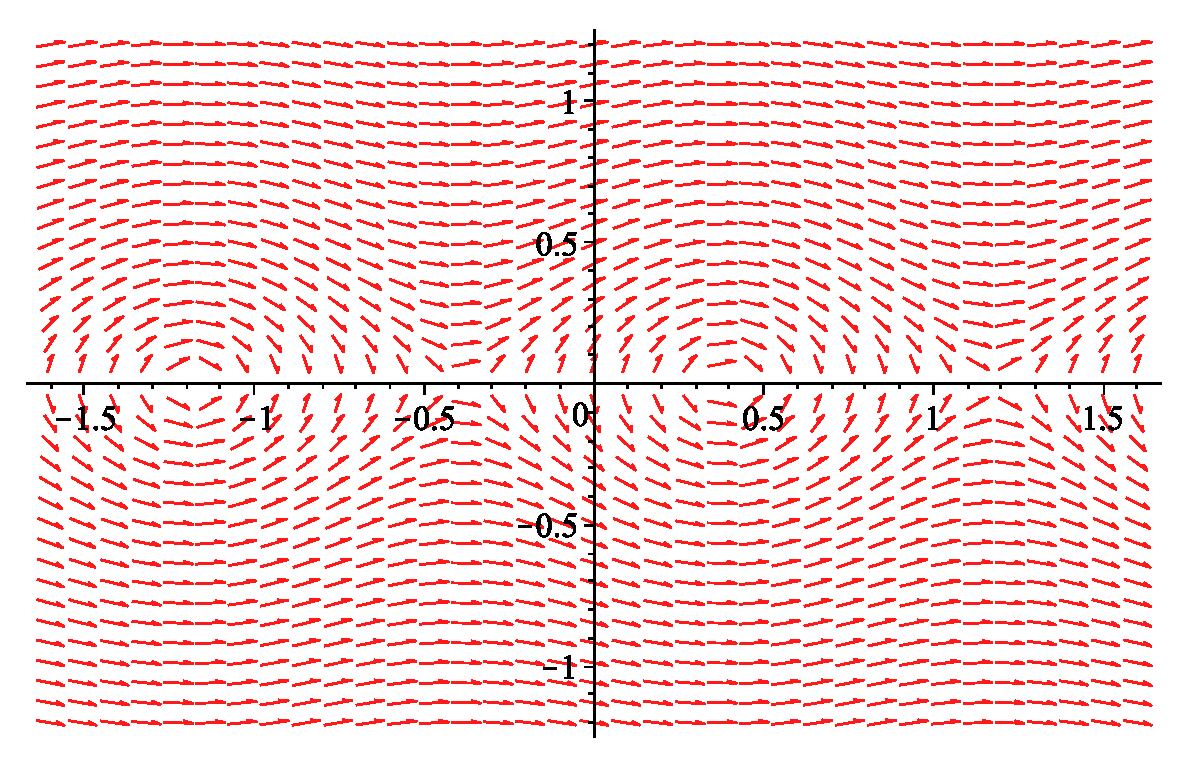
\includegraphics[width=.5 \textwidth]{IVP.eps}
\end{figure}

\item[II.] Based on the direction field, does it look like the solution is defined for all real $x$ for any choice of $a>0$?
\item[III.] Solve the initial value problem $\dfrac{dy}{dx} = \dfrac{\cos(3x)}{3y}, ~ ~ ~ ~ y(0)=a$.  Explicitly solve for $y$ in your final answer.
\item[IV.] Find the smallest value for $a$ for which the solution is defined for all real $x$.
\end{itemize}

\begin{solution}
II. No, in particular the solution for $a=\frac{1}{10}$ does not appear to exist for all $x$. 

III. Separating variables, we have
$$
\int 3y \d y = \int \cos (3x) \d x.
$$
Taking antiderivatives, we have
$$
\frac{3}{2}y^2 = \frac{1}{3} \sin(3x) + C.
$$
Solving for $y$ yields
$$
y = \pm \sqrt{\frac{2}{9} \sin(3x) + C}.
$$
Since $a > 0$, we take the positive solution and solve for $C$ as
$$
a = \sqrt{C} \Rightarrow C = a^2.
$$
Therefore the general solution is
$$
y = \sqrt{\frac{2}{9} \sin(3x) + a^2}.
$$

IV. The smallest positive value of $a$ for which $y$ is defined for all $x$ must satisfy
$$
\frac{2}{9} \sin(3x) + a^2 \geq 0
$$
for all $x$. Since the minimimum value of $\sin(3x)$ is $-1$, the parameter $a$ must satisfy
$$
-\frac{2}{9} + a^2 \geq 0,
$$
or 
$$
a \geq \sqrt{\frac{2}{9}} \approx 0.47.
$$
\end{solution}
\end{problem}


%%%%%%%%%%%%%%%%%%%%%%%%%
\begin{problem} 

Consider the IVP:  $$\dfrac{dy}{dt} = 2y(y-2), ~ ~ ~ ~ y(0)=b.$$

\begin{itemize}
\item[I.] The direction field for the differential equation is shown below.  Based off of this, for initial conditions should the longterm solution stay finite, that is, for which $b$ will $\lim_{t \to \infty} y(t)$ be finite?

 \begin{figure}[h!]
 \centering
  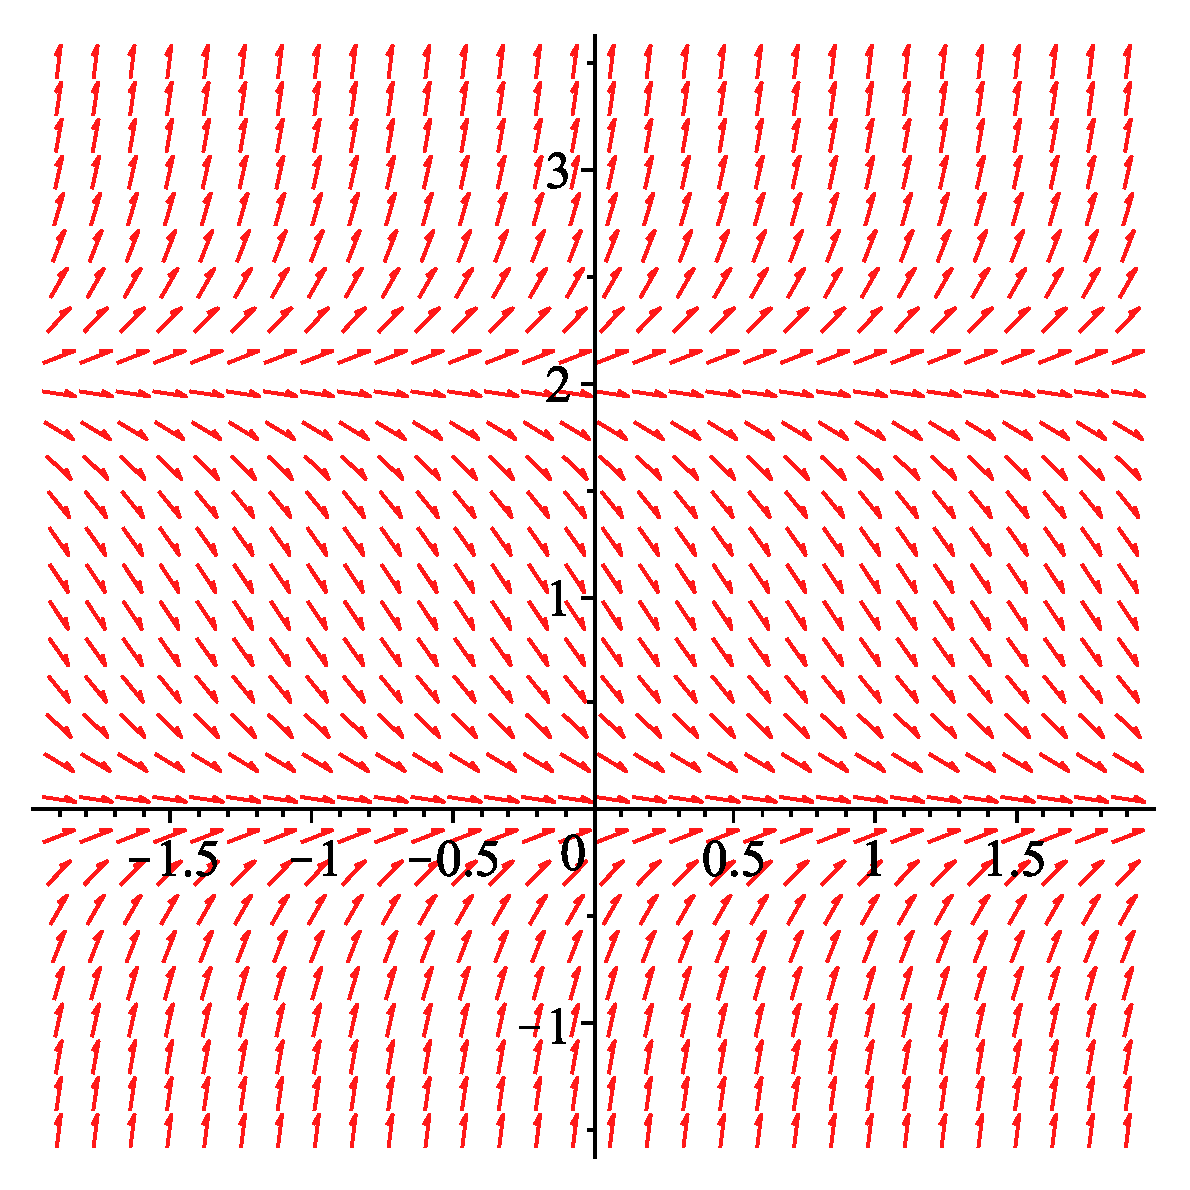
\includegraphics[width=.5 \textwidth]{IVP2.eps}
\end{figure}

\item[II.] Solve the initial value problem $\dfrac{dy}{dt} = 2y(y-2)$, $y(0)=b.$ for both $b=1$ and $b=3$.  Explicitly solve for $y$ in your final answer.  
\item[III.] Is  $\lim_{t \to \infty} y(t)$ finite if $b=1$?  What if $b=3$?
\end{itemize}

\begin{solution}
I. It appears that the longterm solutions stays finite when $b > 0$. 

II. Separating variables, we have
$$
\int \frac{1}{2y(y-2)} \d y = \int \d t.
$$
The integral on the lefthand side can be solved via a partial fraction decomposition:
$$
\int \frac{1}{2y(y-2)} \d y = \int \frac{-1/2}{2y} + \frac{1/4}{y-2} \d y = -\frac{1}{4} \ln |y| + \frac{1}{4} \ln |y-2| + C = \ln \left|\frac{y-2}{y}\right|^{1/4} + C.
$$
Our equation therefore becomes
$$
\ln \left|\frac{y-2}{y}\right|^{1/4} = t + C.
$$
Solving for $y$, we have
\begin{align*}
\left|\frac{y-2}{y}\right|^{1/4} = C e^t &\Rightarrow \frac{y-2}{y} = C e^{4t} \\
&\Rightarrow 1- \frac{2}{y} = Ce^{4t} \\
&\Rightarrow y = \frac{2}{1 - C e^{4t}}.
\end{align*}
For $b= 1$, we have
$$
1 = y(0) = \frac{2}{1-C} \Rightarrow 1-C = 2 \Rightarrow C = -1,
$$
so the solution is 
$$
y= \frac{2}{1+e^{4t}}.
$$
For $b=3$, we have 
$$
3 = y(0) = \frac{2}{1-C} \Rightarrow 3-3C = 2 \Rightarrow 1=3C \Rightarrow C = \frac{1}{3},
$$
and the solution is
$$
y = \frac{2}{1-\frac{1}{3} e^{4t}}.
$$

III. The solution for $b=1$ stays finite, with $\lim_{t\rightarrow \infty} y(t) = 0$. The solution for $b=3$ does not stay finite. It has a vertical asymptote where
$$
1-\frac{1}{3} e^{4t} = 0,
$$
which is at 
$$
t= \frac{1}{4} \ln (3).
$$
\end{solution}
\end{problem}






\end{document}
